\documentclass[11pt]{article}
\usepackage[T1]{fontenc}
\usepackage{lmodern}
\usepackage[margin=1.1in]{geometry}
\usepackage{amsmath,amssymb}
\usepackage{graphicx}
\usepackage{booktabs}
\usepackage{xcolor}
\usepackage{mdframed}
\usepackage{enumitem}
\usepackage{parskip}
\usepackage{hyperref}
\hypersetup{colorlinks=true, linkcolor=blue!55!black, urlcolor=blue!55!black}
\linespread{1.06}

\newcommand{\norm}[1]{\lVert #1 \rVert}

\graphicspath{{figures/}}

\newmdenv[linecolor=blue!35!black,backgroundcolor=blue!4,linewidth=0.6pt,
  skipabove=9pt,skipbelow=9pt,innertopmargin=7pt,innerbottommargin=7pt]{intuition}
\newmdenv[linecolor=red!45!black,backgroundcolor=red!4,linewidth=0.8pt,
  skipabove=9pt,skipbelow=9pt,innertopmargin=7pt,innerbottommargin=7pt]{key}
\newcommand{\analogy}[1]{\par\smallskip\noindent\textit{Analogy:} #1\par\smallskip}

\title{\textbf{How We Recovered the Digit}\\[6pt]
{\large A Plain-English Lesson on the ERT Project ---\\
read it start to finish, nothing skipped}}
\author{Travis Whitney \quad\textbar\quad AI 539 \quad\textbar\quad Project 1 group guide}
\date{Spring 2026}

\begin{document}
\maketitle

\begin{quote}
\small This guide is written so that anyone in the group can \emph{understand}
the project well enough to explain it to someone else. We do not assume you
remember the lectures. Every new word is defined the moment it appears, and
every idea is built on the one before it. It is long on purpose: we would
rather over-explain than leave you stuck. Read it in order.
\end{quote}

\tableofcontents
\newpage

%==============================================================
\part*{Part I --- What is the problem?}
\addcontentsline{toc}{section}{Part I --- What is the problem?}
%==============================================================

\section{Lesson 1: What is ERT, in plain terms?}

Imagine a shallow rectangular tray of some material, and you want to know
what is hidden inside it --- but you are not allowed to cut it open or look
inside. All you can do is touch the \emph{edges}.

ERT (\textbf{E}lectrical \textbf{R}esistance \textbf{T}omography) is a way to
``see'' inside using electricity. Around the edge of the tray we place little
metal contacts called \emph{electrodes}. Then we do many small experiments.
In each one we:

\begin{enumerate}[leftmargin=2em]
\item push a tiny electric current in through one electrode and let it come
out another, and
\item measure the voltage (the ``electrical pressure'') at other electrodes
around the edge.
\end{enumerate}

Why does this tell us anything about the inside? Because electricity does not
flow the same way through everything. It zips easily through some materials
and struggles through others. So the pattern of voltages we read at the edge
\emph{depends on what is inside}. If we do enough of these little experiments
and write down all the voltage readings, that big list of numbers secretly
contains information about the hidden interior.

\analogy{It is like a medical CT scan, but instead of X-rays passing through
your body, we use electric current passing through the tray. We never see
inside directly; we only get edge readings and have to figure out the inside
from them.}

In our project the ``hidden thing inside'' is a \textbf{handwritten digit}
(like the ones in the famous MNIST dataset of 0--9 digits). The digit is
``drawn'' in the tray as a region that conducts electricity differently from
its surroundings. Our whole job is: \emph{from the edge voltage readings,
figure out which digit is inside and draw it.}

\section{Lesson 2: The hidden image is just a grid of numbers}

We represent the inside of the tray as a $28\times28$ grid of little squares,
called \emph{pixels} (just like a low-resolution photo). Each pixel holds one
number: how well electricity flows at that spot. That number is called the
\textbf{conductivity}.

\begin{itemize}[leftmargin=2em]
\item A \emph{high} conductivity number = electricity flows easily there
(think copper wire).
\item A \emph{low} conductivity number = electricity struggles there
(think rubber).
\end{itemize}

So ``the hidden image'' is literally a grid of $28\times28 = 784$ numbers. The
background (empty tray) has a baseline conductivity --- in our setup, the
number $1$ everywhere. The digit is drawn as pixels whose conductivity is
\emph{higher} than $1$. When you look at a picture of the answer, bright
pixels = high conductivity = the strokes of the digit; dark pixels =
background.

\begin{intuition}
Whenever we say ``the image'' or ``the conductivity image'' or use the symbol
$\sigma$ (Greek letter ``sigma''), we just mean this grid of 784 numbers. It
is the thing we are trying to find. We often stack the grid into one tall
column of 784 numbers so we can do math with it; that does not change
anything, it is just bookkeeping.
\end{intuition}

\section{Lesson 3: ``Forward'' vs.\ ``Inverse'' --- the heart of everything}

There are two directions you can go.

\textbf{The forward direction (easy).} Suppose someone hands you the image
$\sigma$ (you know exactly what is inside). Then a computer can simulate the
physics and tell you \emph{what the edge voltage readings would be}. Image in,
readings out. There is no guesswork --- it is just a simulation.

\textbf{The inverse direction (hard).} Now flip it around. You are \emph{not}
given the image. You are only given the edge readings, and you must work
backward to figure out the image that produced them. Readings in, image out.
This is our actual problem, and it is much harder.

\analogy{Forward: you have a recipe, you follow it, you get a cake. Easy and
certain. Inverse: someone hands you a cake and you must figure out the exact
recipe. Much harder --- maybe several recipes could make a nearly identical
cake, and a tiny change in how it tastes might come from many different
ingredient tweaks. That ``many recipes give nearly the same cake'' problem is
exactly what makes our task hard, as we will see.}

\section{Lesson 4: The forward simulator, $F$}

We give the forward simulator a name: $F$. Think of $F$ as a black box:

\[
\text{(an image $\sigma$, 784 numbers)} \;\longrightarrow\; \boxed{\,F\,}
\;\longrightarrow\; \text{(the edge readings $y$, 1900 numbers)} .
\]

We write this as $y = F(\sigma)$: ``$y$ is what you get when you run the
simulator $F$ on the image $\sigma$.'' In our project the readings $y$ are a
list of 1900 numbers (we did many little current experiments, each producing
several voltage readings, and stacked them all together).

\paragraph{What is inside the black box (the gentle version).} You do not need
this to follow the rest, but here is the gist. Physicists have an equation
describing how electric voltage spreads through a material. It says, roughly,
``electric charge is conserved, and current flows from high voltage to low
voltage at a rate set by the conductivity.'' The simulator takes your image,
applies that rule everywhere on the grid, solves a big system of linear
equations to find the voltage at every pixel, and then reads off the voltages
at the edge electrodes. That is $F$. The code that does this is the file
\texttt{ERT2D.m}; we treat it as a trustworthy black box.

\begin{figure}[h]\centering
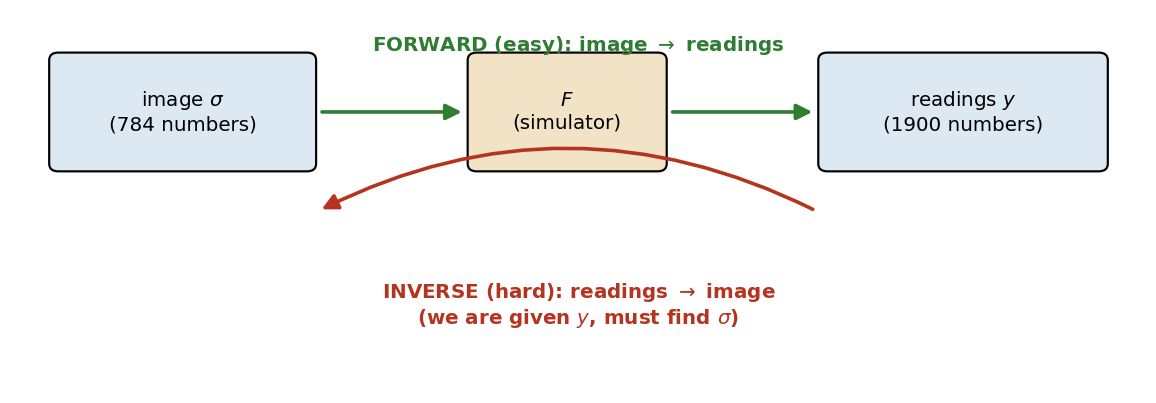
\includegraphics[width=0.95\textwidth]{fig_forward_inverse.png}
\caption{The two directions. Forward (green) is a simulation: image in,
readings out --- easy and certain. Inverse (red) is our job: readings in,
image out --- hard, because we have to undo the simulation.}
\end{figure}

\begin{key}
The whole project in one line:
\[
\underbrace{\sigma}_{\text{image we WANT (784 numbers)}}
\;\xrightarrow{\ F\ }\;
\underbrace{y}_{\text{readings we HAVE (1900 numbers)}}.
\]
We are given the right-hand side and must find the left-hand side.
\end{key}

\begin{intuition}
\textbf{Explain it to a friend in 60 seconds (Part I).} ``We have a box. We
can't look inside, but we can run little electrical experiments on its edges
and get 1900 voltage readings. Those readings depend on what's inside, which
is a handwritten digit drawn in `how-easily-electricity-flows.' Running the
simulation \emph{forward} (digit $\to$ readings) is easy. We have to go
\emph{backward} (readings $\to$ digit), which is the hard part.''
\end{intuition}

%==============================================================
\part*{Part II --- Why is this so hard?}
\addcontentsline{toc}{section}{Part II --- Why is this so hard?}
%==============================================================

\section{Lesson 5: Hard reason \#1 --- many different images give almost the same readings}

Here is the first thing that makes the inverse problem nasty. \emph{Very
different} hidden images can produce \emph{nearly identical} edge readings.

Why? Because the edge electrodes are far from the fine details inside. By the
time the effect of a small interior feature reaches the edge, it has been
blurred and averaged out with everything else. The edge only sees a smeared
summary of the interior. Fine details --- exactly the things that tell a ``3''
apart from a ``5'' --- barely register at the edge.

\analogy{Think of a shadow on a wall. Many different 3D objects can cast
almost the same shadow. If all you have is the shadow, you cannot be sure
which object made it. Here, the edge readings are like a shadow of the
interior: lots of different interiors cast nearly the same ``electrical
shadow.''}

So if we only insist ``find an image whose readings match,'' there are
\emph{tons} of images that fit --- including ugly, meaningless, static-looking
ones. Matching the readings is not enough to pin down the answer.

\section{Lesson 6: Hard reason \#2 --- tiny measurement errors blow up}

Real measurements are never perfect; every reading is off by a tiny amount
(we will call this \emph{noise} in Lesson 7). Normally a tiny error would be
no big deal. But for this kind of problem, tiny errors in the readings can
cause \emph{huge} errors in the recovered image.

Here is the intuition. Going forward, $F$ \emph{blurs} the interior. Going
backward means \emph{un-blurring}. And un-blurring is dangerous: to undo a
blur you essentially have to ``divide by very small numbers,'' and dividing by
something tiny makes things explode. A microscopic wiggle in the readings,
divided by a tiny number, becomes a giant wiggle in the image.

\analogy{Imagine someone whispers a long number to you across a noisy room,
and you have to multiply what you heard by a million. If you mishear by even a
little, your final answer is off by millions. The ``multiply by a million''
step is what un-blurring does to measurement noise.}

\paragraph{The name for all this.} A problem where (a) the answer is not
unique, and/or (b) tiny data errors cause huge answer errors, is called
\textbf{ill-posed}. Our problem is badly ill-posed on both counts. This single
fact is \emph{why} the project is interesting and why naive approaches fail.

\begin{key}
Because the problem is ill-posed, ``just find an image whose readings match''
is hopeless --- the answer is not unique and is wildly sensitive to noise. We
need to add \emph{extra knowledge} about what the answer should look like.
That extra knowledge is called a \textbf{prior}, and getting it right is the
whole game. The next part builds up exactly what a prior is.
\end{key}

\begin{intuition}
\textbf{Explain it to a friend in 60 seconds (Part II).} ``It's hard for two
reasons. First, lots of different digits produce almost the same edge readings
--- like how many objects can cast the same shadow --- so the readings don't
point to a single answer. Second, the readings are slightly noisy, and undoing
the blur magnifies that noise enormously. So `find any image that matches the
readings' gives garbage. We need to tell the method what a real answer should
look like.''
\end{intuition}

%==============================================================
\part*{Part III --- Turning ``recover the image'' into a math problem}
\addcontentsline{toc}{section}{Part III --- Turning the goal into a math problem}
%==============================================================

This part is the conceptual core. We slowly turn the vague goal ``find the
right image'' into a precise recipe a computer can chase. We build it in
small pieces: noise, then ``likelihood,'' then ``why squared error,'' then
``prior,'' then how to combine them.

\section{Lesson 7: Measurement noise}

When you measure anything in the real world, the number you get is the true
value plus a little random error. A thermometer reads $70.2^\circ$ when the
room is really $70.0^\circ$. That $0.2$ is \emph{noise}: a small, random,
unpredictable wobble.

Our 1900 readings each have a little noise on them. We write this as
\[
\text{(what we measured)} = \text{(true readings)} + \text{(noise)} .
\]
The standard assumption --- and a reasonable one --- is that this noise follows
the famous \textbf{bell curve} (the ``Gaussian'' or ``normal''
distribution): small wobbles are common, big wobbles are rare, and it is just
as likely to be a bit high as a bit low. Picture the classic bell shape:
tall in the middle (near zero error), tailing off on both sides.

\begin{intuition}
You do not need any formula yet. Just hold onto two facts: (1) every reading
is a little off, and (2) ``a little off'' is common while ``way off'' is rare
--- that is what the bell curve means.
\end{intuition}

\section{Lesson 8: ``Likelihood'' --- the key idea, taught with a guessing game}

This is the most important concept in the whole project, so we build it
slowly with a game that has nothing to do with electricity.

\paragraph{The game.} I think of a secret number. I run it through a simple
machine: ``multiply by 2.'' Then I add a small random wobble (noise). I tell
you the result is $14.2$. Your job: guess my secret number.

Your gut probably says ``about $7$,'' because $7\times2 = 14$, which is close
to $14.2$. Good. But let us turn that gut feeling into something precise,
because that precise version is exactly what we will use for the real problem.

\paragraph{The precise question.} For \emph{any} guess, ask: ``\emph{If my
guess were right, how believable is the result I actually saw?}''

\begin{itemize}[leftmargin=2em]
\item Guess $= 7$. Then the machine outputs $14$, so the wobble needed to
reach $14.2$ is just $0.2$. A wobble of $0.2$ is small --- totally believable
(near the top of the bell curve). So guess $7$ scores \emph{high}.
\item Guess $= 6$. The machine outputs $12$, so the wobble needed is $2.2$.
That is a biggish wobble --- less believable (partway down the bell). Guess $6$
scores \emph{lower}.
\item Guess $= 100$. The machine outputs $200$, so the wobble needed is
$-185.8$. A wobble that gigantic is absurd (way out in the flat tail of the
bell). Guess $100$ scores essentially \emph{zero}.
\end{itemize}

That score --- ``how believable is the data I saw, if this guess were the
truth'' --- has a name: the \textbf{likelihood} of the guess. The best guess is
the one with the highest likelihood. Here, that is $7$ (give or take a hair),
matching your gut.

\begin{figure}[h]\centering
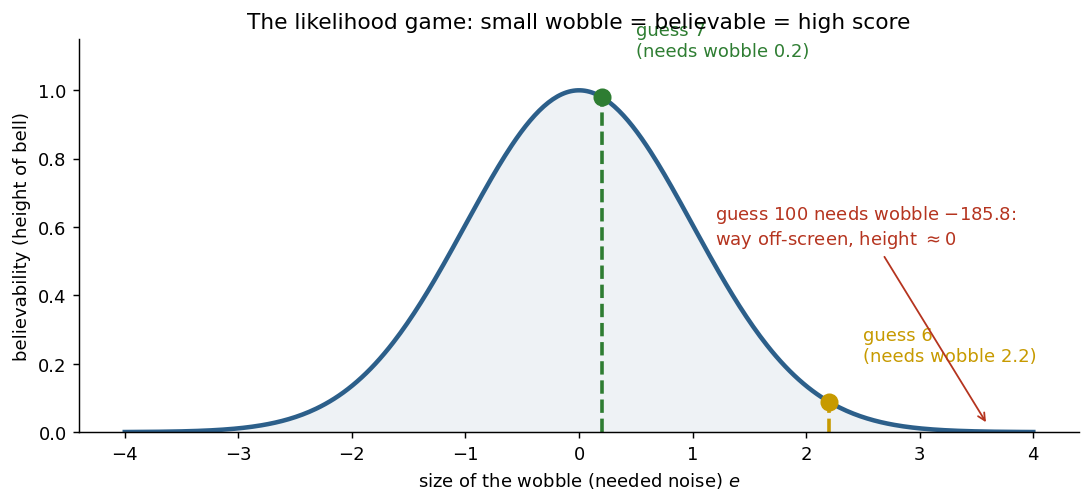
\includegraphics[width=0.85\textwidth]{fig_likelihood.png}
\caption{The guessing game on the bell curve. Each guess needs a certain
wobble to explain the data ($14.2$); we read that wobble's believability off
the bell. Guess 7 needs a tiny wobble (high score, green); guess 6 needs a
bigger one (lower score); guess 100 needs an absurd wobble (essentially zero).}
\end{figure}

To make ``score'' concrete, here are the actual heights of the bell at each
needed wobble (using the bell's height formula $e^{-e^2/2}$ from Lesson 9 ---
you do not need to compute these by hand, just see the pattern):
\begin{center}
\begin{tabular}{cccc}
\toprule
guess & machine output & needed wobble $e$ & likelihood (bell height) \\
\midrule
$7$   & $14$  & $0.2$    & $0.98$ \quad(almost the max)\\
$6$   & $12$  & $2.2$    & $0.09$ \quad(small)\\
$100$ & $200$ & $-185.8$ & $\approx 10^{-7480}$ \quad(basically zero)\\
\bottomrule
\end{tabular}
\end{center}
Guess 7 wins by a mile. The numbers just make precise what your gut already
knew: the guess whose prediction is closest to what we saw is the most
believable.

\begin{key}
\textbf{Likelihood} = ``if this candidate answer were the truth, how believable
is the data we actually measured?'' We score every candidate this way and
prefer the candidate with the highest score. Picking the highest-likelihood
candidate is called \textbf{maximum likelihood}. \emph{This is the engine
behind turning our problem into an optimization.}
\end{key}

\paragraph{Back to ERT.} Exactly the same idea. A ``candidate'' is now a
candidate image $\sigma$. The ``machine'' is the forward simulator $F$. For a
candidate image, the wobble needed to explain the data is
\[
\text{needed noise} = \underbrace{y_{\text{obs}}}_{\text{what we measured}}
- \underbrace{F(\sigma)}_{\text{what this candidate predicts}} .
\]
If the candidate's predicted readings $F(\sigma)$ are close to the measured
readings $y_{\text{obs}}$, the needed noise is small and believable
$\Rightarrow$ high likelihood. If they are far apart, the needed noise is
huge and unbelievable $\Rightarrow$ tiny likelihood. We want the image with
the highest likelihood.

\section{Lesson 9: Why we end up ``minimizing squared error''}

You will constantly hear the phrase ``least squares'' or ``minimize the
squared error.'' Let us see \emph{why} that specific thing falls out of
Lesson 8 --- it is not arbitrary.

The bell curve has a specific shape. Written as a formula, the believability
of a wobble of size $e$ is proportional to
\[
\exp\!\Big(-\tfrac{e^2}{2\,(\text{noise size})^2}\Big),
\]
where $\exp$ is the exponential function. You do not need to memorize this.
The only thing that matters is what is \emph{inside}: the wobble gets
\textbf{squared} ($e^2$), and there is a minus sign.

Now, for our many readings at once, the total believability multiplies
together (more on ``multiply'' in Lesson 21), and a standard trick is to take
the \emph{logarithm}, which turns the exponential into just its exponent and
turns multiplication into addition. After that trick, ``maximize
believability'' becomes ``\emph{minimize} the sum of squared wobbles'':
\[
\text{minimize}\quad
\underbrace{\big(F(\sigma) - y_{\text{obs}}\big)\text{'s, each squared, summed up}}_{\textstyle =\ \norm{F(\sigma)-y_{\text{obs}}}^2} .
\]
The notation $\norm{v}^2$ just means ``square every number in the list $v$ and
add them up.'' The list here is the \emph{residual} $r = F(\sigma) -
y_{\text{obs}}$: reading-by-reading, how far off our candidate's prediction is
from the measurement.

\begin{intuition}
\textbf{Why square, instead of just adding up the errors?} Two reasons.
(1) Squaring makes every error positive, so a $+3$ error and a $-3$ error do
not secretly cancel to ``zero error'' --- both count as bad. (2) Squaring
punishes big misses much more than small ones, which is exactly what the bell
curve says (big wobbles are very unlikely). The squared form is the
mathematical fingerprint of ``the noise is a bell curve.''
\end{intuition}

\begin{key}
``Minimize $\tfrac12\norm{F(\sigma)-y_{\text{obs}}}^2$'' (the \textbf{data
term}) is just a precise way of saying ``find the image whose predicted
readings best match the measured readings, assuming bell-curve noise.'' It is
maximum likelihood in disguise. \emph{But} --- from Part II --- this alone is
not enough, because many images match. We need a prior.
\end{key}

\section{Lesson 10: A ``prior'' --- what you believe before looking at the data}

A \textbf{prior} is your belief about the answer \emph{before} you take the
measurements into account. It encodes ``what does a plausible answer even look
like?''

\analogy{A friend says ``I scored 100\% on the exam.'' How much do you believe
them? It depends on your \emph{prior}: if the exam was famously brutal, you are
skeptical; if it was easy, you readily believe. Same statement, different
conclusion, because your prior belief differs. A prior is exactly this
``before-the-evidence'' belief, and it genuinely changes the final answer.}

For our problem, the prior answers: ``of all the $784$-number images that
could possibly fit the readings, which ones are \emph{believable as an
answer}?'' A prior that says ``the answer should look like a handwritten
digit'' is enormously more useful than no prior at all, because it throws out
all the static-looking junk images that happen to match the readings.

\begin{intuition}
This is where Part II's trouble gets fixed. The readings alone cannot choose
between the many images that fit (ill-posedness). The prior breaks the tie by
saying ``...and of those, prefer the ones that actually look like a digit.''
The better your prior, the better your answer. Most of this project is a
contest between different priors.
\end{intuition}

\section{Lesson 11: Combining the two --- and the big unifying idea}

We have two ingredients:
\begin{itemize}[leftmargin=2em]
\item the \textbf{data term} (Lesson 9): prefer images whose readings match,
and
\item the \textbf{prior} (Lesson 10): prefer images that look like plausible
answers.
\end{itemize}
The recipe is to add them and minimize the total:
\[
\text{best image} \;=\; \text{the image that minimizes}\quad
\underbrace{\tfrac12\norm{F(\sigma)-y_{\text{obs}}}^2}_{\text{match the data}}
\;+\;
\underbrace{\lambda\, R(\sigma)}_{\text{look like a plausible answer}} .
\]
Here $R(\sigma)$ is a \emph{penalty} that is small for ``good-looking'' images
and large for ``bad-looking'' ones --- it is the prior, written as a cost. The
number $\lambda$ (``lambda'') is a knob that sets how much we care about the
prior versus the data. Big $\lambda$: trust the prior a lot. Small $\lambda$:
trust the data a lot. This penalty $R$ is called the \textbf{regularizer}.

\begin{key}
\textbf{The single most important idea in the project:} a \emph{regularizer is
just a prior in disguise}. Choosing a penalty $R(\sigma)$ is exactly the same
as choosing what you believe a good answer looks like. Every method we tried
--- Tikhonov, $\ell_1$, TV, PCA, the VAE, and the winning template method ---
is nothing more than a \emph{different choice of prior}. Once you see this, the
whole project becomes one question: \emph{what is the best prior?}
\end{key}

%==============================================================
\part*{Part IV --- How the computer actually searches}
\addcontentsline{toc}{section}{Part IV --- How the computer searches}
%==============================================================

We have a thing to minimize. Now, how does a computer find the minimum? It
walks downhill. This part explains how, in plain terms.

\section{Lesson 12: The gradient --- which way is downhill}

Picture the quantity we want to minimize as a \emph{landscape}: every possible
image is a location, and the height at that location is how bad that image is
(big penalty + bad data match = high ground; the perfect answer = the lowest
valley). We want to reach the bottom.

The \textbf{gradient} is simply the arrow that points \emph{straight uphill}
from wherever you are standing, and its length says how steep the slope is. So
to go \emph{down}, you step in the \emph{opposite} direction of the gradient.

\analogy{You are on a foggy hillside and want to reach the valley. You cannot
see far, but you can feel which way the ground slopes under your feet. You take
a step downhill, feel again, step again. That is \textbf{gradient descent}:
repeatedly ``feel the slope, step downhill.'' The gradient is the ``feel the
slope'' part.}

\begin{figure}[h]\centering
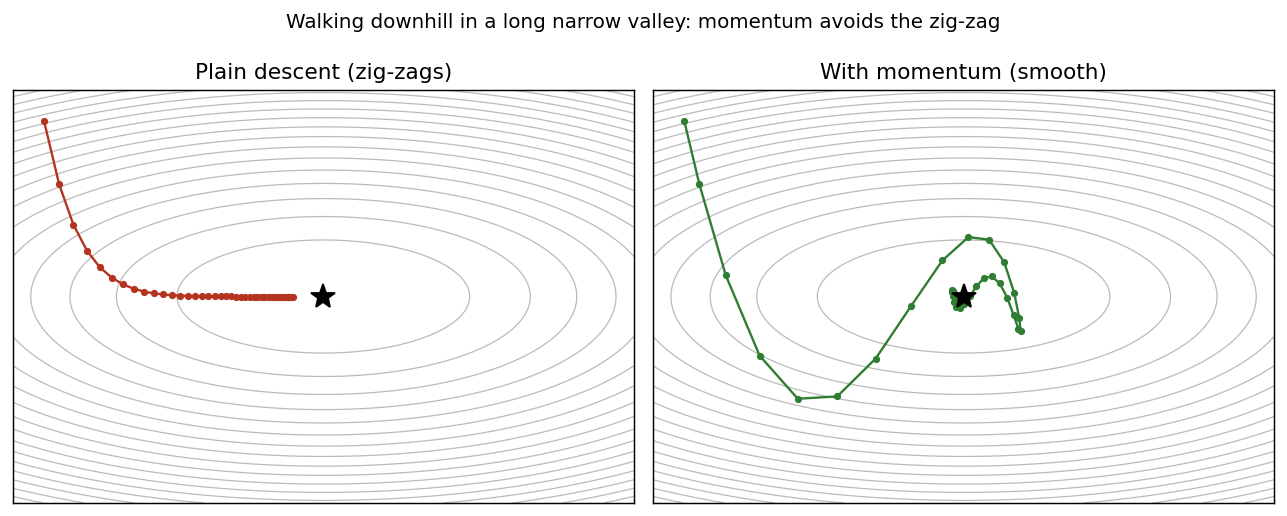
\includegraphics[width=0.95\textwidth]{fig_gd_momentum.png}
\caption{Walking downhill toward the lowest point (the star). In a long, narrow
valley, plain stepping (left) zig-zags wastefully across the valley. Momentum
(right) remembers recent steps and rolls smoothly to the bottom. We will need
this picture again in Lesson 14.}
\end{figure}

\section{Lesson 13: The gradient of our problem ($J^\top r$), explained}

To walk downhill we need the gradient of the data term. It turns out to have a
clean, meaningful form. Two pieces go into it.

\textbf{Piece 1: the residual $r$.} This is the list of how wrong our current
guess is at each of the 1900 readings: $r = F(\sigma) - y_{\text{obs}}$. Big
$r_i$ means ``reading $i$ is badly mismatched right now.''

\textbf{Piece 2: the sensitivity table $J$ (the ``Jacobian'').} This is a big
table that answers, for every pair (reading $i$, pixel $j$): ``if I brighten
pixel $j$ a tiny bit, how much does reading $i$ change?'' That single number
is the entry $J_{ij}$. The whole table $J$ thus describes how every pixel
influences every reading.

Now, the gradient (call it ``which pixels to change, and how much'') is built
by, for each pixel, going through all 1900 readings and adding up:
\[
(\text{how wrong reading } i \text{ is}) \times
(\text{how much pixel } j \text{ affects reading } i),
\]
summed over all readings $i$. In compact notation this sum is written
$J^\top r$ (the little ``$\top$'' means we use the table ``sideways,'' reading
it pixel-by-pixel instead of reading-by-reading).

\begin{intuition}
\textbf{Read $J^\top r$ as a weighted vote.} Each reading gets a vote on how to
change each pixel. A reading that is currently very wrong (big $r_i$) votes
loudly; a reading that already matches (small $r_i$) barely votes. And each
reading pushes hardest on the pixels it is most sensitive to. Add up all the
votes and you get: ``the pixels that most strongly affect the most-wrong
readings should change the most.'' That is the downhill direction.
\end{intuition}

\paragraph{A tiny worked example (do this one by hand).} Pretend there are
just 2 readings and 2 pixels. Suppose right now our residual (how wrong each
reading is) is
\[
r = \begin{pmatrix} r_1 \\ r_2 \end{pmatrix}
  = \begin{pmatrix} 2 \\ 1 \end{pmatrix}
  \qquad(\text{reading 1 is off by }2,\ \text{reading 2 is off by }1),
\]
and the sensitivity table is
\[
J = \begin{pmatrix} J_{11} & J_{12} \\ J_{21} & J_{22}\end{pmatrix}
  = \begin{pmatrix} 4 & 1 \\ 2 & 3 \end{pmatrix}
\]
(e.g.\ $J_{11}=4$ means ``pixel 1 strongly affects reading 1''). The gradient
entry for \emph{pixel 1} sums, over the readings, (how wrong) $\times$ (how
much pixel 1 affects that reading):
\[
(J^\top r)_1 = \underbrace{r_1 J_{11}}_{2\cdot 4} + \underbrace{r_2 J_{21}}_{1\cdot 2}
= 8 + 2 = 10 .
\]
For \emph{pixel 2}:
\[
(J^\top r)_2 = \underbrace{r_1 J_{12}}_{2\cdot 1} + \underbrace{r_2 J_{22}}_{1\cdot 3}
= 2 + 3 = 5 .
\]
So the gradient is $\binom{10}{5}$: pixel 1 should change twice as much as
pixel 2, because pixel 1 has more influence on the readings that are most
wrong. That is the entire meaning of $J^\top r$ --- a weighted tally, nothing
more mysterious.

\paragraph{(Optional aside) Why computing $J$ is not impossibly slow.} The
table $J$ has $1900\times784$ entries. Computing it the dumb way --- nudge each
of the 784 pixels and re-run the whole simulation --- would mean 784
simulations per step, far too slow. There is a beautiful shortcut called the
\emph{adjoint method} that gets the entire table with essentially \emph{two}
simulations instead of 784: one ``forward'' run (push current from the source)
and one ``backward'' run (pretend to push current from the sensor). A pixel
matters wherever those two flows overlap. You do not need the details to
present the project --- just know that this trick is what makes the whole thing
fast enough to run, and it is already done for us inside \texttt{ERT2D.m}.

\section{Lesson 14: Gradient descent, with a little ``momentum''}

So the basic algorithm is: feel the slope ($J^\top r$ plus the prior's slope),
take a small step downhill, repeat. The step size is a number $\eta$ (``eta'')
called the \emph{learning rate}: too big and you overshoot the valley and
bounce around; too small and you crawl forever.

One upgrade makes it much faster on our problem. Because the landscape is a
long, narrow valley (a side effect of ill-posedness), plain downhill stepping
zig-zags across the valley and inches along it. The fix is \textbf{momentum}:
instead of basing each step only on the current slope, you keep a running
``velocity'' that remembers recent steps, like a ball rolling downhill that
builds up speed. The zig-zags cancel out and the ball powers along the valley.

\analogy{A marble rolling down a curved gutter does not stop and re-decide its
direction at every inch --- it carries momentum and smoothly follows the
gutter to the bottom. Momentum gives our search that same smoothness.}

(The figure back in Lesson 12 shows exactly this: left panel is the zig-zag of
plain stepping; right panel is the smooth momentum path to the bottom.)

That is the entire optimization toolkit. Every method below uses this same
``roll downhill with momentum'' loop; they differ only in the prior.

\begin{intuition}
\textbf{Explain it to a friend in 60 seconds (Parts III--IV).} ``We turned
`recover the image' into `find the image that minimizes (how badly its
predicted readings miss the real ones) plus (how unlike a real answer it
looks).' The first part comes from assuming bell-curve noise; the second part
is the \emph{prior}, and choosing a prior \emph{is} choosing what you believe.
Then the computer just walks downhill --- nudging the image in the direction
$J^\top r$ (a weighted vote where the most-wrong readings push hardest on the
pixels they care about), using momentum so it doesn't zig-zag.''
\end{intuition}

%==============================================================
\part*{Part V --- What we tried, and why each behaved as it did}
\addcontentsline{toc}{section}{Part V --- What we tried, and why each behaved as it did}
%==============================================================

Now the fun part: a tour of the priors we tried, from crudest to smartest,
and exactly why each one succeeded or failed. Remember (Lesson 11): each
method is just a different belief about ``what a good answer looks like.''

\section{Lesson 15: Tikhonov --- ``keep it small and smooth''}

The simplest prior says: ``prefer images whose pixel values are small and
gently varying.'' Its penalty $R$ adds up the \emph{squares} of the pixel
values, so any large value is punished hard.

\textbf{What happens.} Because big values are punished so heavily, the method
avoids committing to bright, sharp strokes. Instead it spreads a little bit of
brightness over a wide area --- a faint, blurry smudge. You can sort of see
``something is in the middle,'' but never an actual digit. This is the starter
code's behavior, and no setting of the knob $\lambda$ fixes it: the prior
fundamentally wants smooth blandness, and a digit is neither smooth nor bland.

\section{Lesson 16: $\ell_1$ --- ``most pixels should be exactly blank''}

A digit is mostly empty: the strokes occupy a minority of pixels, and the rest
is pure background. The $\ell_1$ (``ell-one'') prior captures ``mostly blank''
by adding up the \emph{plain sizes} (absolute values) of the pixel values
instead of their squares.

Why does that encourage blankness? Here is the neat part. With squares
(Tikhonov), shrinking a pixel from $0.1$ to $0$ barely reduces the penalty
($0.1^2 = 0.01$ is already tiny), so the method leaves lots of faint nonzero
pixels lying around --- blur. With plain sizes ($\ell_1$), shrinking $0.1$ to
$0$ removes the whole $0.1$ of penalty, so the method is rewarded for setting
weakly-supported pixels to \emph{exactly} zero. The result is a clean,
sparse image: a handful of pixels ``on,'' the rest exactly ``off.''

\analogy{Squares are like a tax that is negligible on small amounts, so you
do not bother clearing out the small stuff. Plain size is a flat fee on
\emph{any} nonzero amount, so you aggressively zero out everything you do not
truly need.}

\begin{figure}[h]\centering
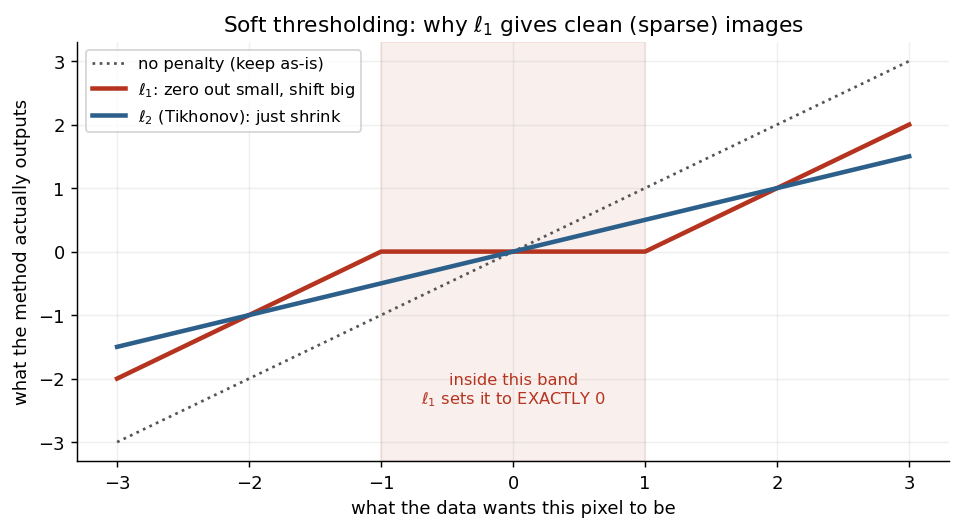
\includegraphics[width=0.78\textwidth]{fig_softthreshold.png}
\caption{What each penalty does to a pixel. Horizontal: what the data alone
wants the pixel to be. Vertical: what the method outputs. $\ell_1$ (red) snaps
anything in the shaded band to \emph{exactly} zero and shifts the rest toward
zero --- giving clean, sparse images. $\ell_2$/Tikhonov (blue) only shrinks
everything a bit, never reaching zero --- giving blur.}
\end{figure}

This behavior has a name: \textbf{soft thresholding}. Concretely, with a knob
$\lambda=1$: if the data wants a pixel to be $0.3$, $\ell_1$ outputs
\emph{exactly} $0$ (it was inside the ``snap to zero'' band); if the data wants
$1.5$, $\ell_1$ outputs $1.5-1=0.5$ (kept, but shrunk). Tikhonov, by contrast,
would output something like $0.15$ and $0.75$ --- everything survives, faintly.
That difference (exact zeros vs.\ faint survivors) is exactly clean-digit
vs.\ blur.

\textbf{What happens for us.} Better than Tikhonov in spirit, but alone it
gives scattered specks rather than a connected digit shape, because it cares
about individual pixels, not whether they form a coherent stroke.

\section{Lesson 17: Total Variation (TV) --- ``few sharp edges''}

A digit is made of solid strokes with sharp boundaries: inside a stroke,
neighboring pixels are the same; you only get a jump at the \emph{edge} of a
stroke. TV captures this by penalizing \emph{differences between neighboring
pixels} (using the same ``plain size'' trick as $\ell_1$, but applied to
neighbor-differences instead of to pixel values).

The effect: TV is happy with large uniform regions (no neighbor differences =
no penalty there) and only pays a cost along edges. So it prefers
\emph{piecewise-flat images with clean boundaries} --- which is roughly what a
digit is. TV was the best of the generic priors, but still came out as a vague
localized region rather than a readable digit: ``few sharp edges'' is closer
to a digit than ``small'' or ``sparse,'' but it still does not know what a
\emph{digit} actually is.

\begin{key}
Tikhonov, $\ell_1$, and TV are all \emph{generic} priors: ``small,''
``sparse,'' ``few edges.'' None of them knows what a handwritten digit looks
like. That is their ceiling. To do better we need a prior that has actually
\emph{seen} digits. That is the next idea.
\end{key}

\section{Lesson 18: The leap --- a prior that learned from real digits}

We have 60{,}000 real MNIST digit images sitting in a file. Why describe a
``good answer'' with a vague word like ``sparse'' when we have 60{,}000
examples of exactly what good answers look like? The next two methods build
the prior \emph{from the data itself}.

The idea: don't let the answer be \emph{any} 784-number image. Force it to be
``the kind of image that looks like the MNIST examples.'' We tried two ways to
do this: a simpler \emph{linear} way (PCA) and a fancier \emph{curved} way
(the VAE). To understand them we first need one new idea: a ``building-block''
representation of images.

\section{Lesson 19: PCA --- building digits from learned building blocks}

\paragraph{Building blocks (a basis).} Here is the key concept. Just as any
paint color can be mixed from a few primary colors, it turns out any
\emph{digit-like} image can be approximated by mixing a small set of special
``building-block images.'' You take building-block \#1, multiply it by some
amount, add building-block \#2 times some amount, and so on. The list of ``how
much of each block'' is a short list of numbers --- say $50$ of them. Mix
according to those 50 numbers and you get an image.

\analogy{A recipe. The building blocks are the ingredients (flour, sugar,
eggs, \dots). The ``how much of each'' numbers are the amounts. Different
amount-lists give different cakes, but every result is recognizably a cake
because you are only ever combining cake ingredients.}

\paragraph{Where do the building blocks come from? (PCA.)} \emph{Principal
Component Analysis} (PCA) is a standard procedure that looks at all 60{,}000
digits and extracts the handful of building-block images that best capture how
digits vary. The first block is roughly the ``average digit''; later blocks
capture the main ways digits differ from that average. Keep the top $K$ blocks
(we used $K$ around 50--150).

\paragraph{How we use it.} Instead of searching over all 784 pixel values
freely, we only search over the $K$ ``how much of each block'' numbers. Every
image we can build is automatically a blend of real-digit building blocks ---
so it cannot become static-looking junk. This both shrinks the search (50
numbers instead of 784) and bakes in the digit prior. (The downhill direction
is still our friend $J^\top r$, just translated into ``how should I change the
50 mixing amounts'' by a bit of bookkeeping.)

\textbf{What happened.} Big improvement! For the first time we got clean,
\emph{digit-shaped} reconstructions, and in fact the \emph{lowest} data-match
error of any method. \emph{But} --- it produced the \emph{wrong digit}. Our
true answer was a ``2'' and PCA confidently returned a ``9.'' Why? That needs
its own lesson.

\section{Lesson 20: Why PCA got the wrong digit --- ``flat sheets'' and many valleys}

Two reasons, and both are worth understanding because they explain a lot.

\paragraph{Reason 1: a flat sheet cannot follow a curved surface.} Think of
all possible images as points in a vast space. The real digits do not fill
this space --- they sit on a thin, \emph{curved} surface within it (most of the
space is meaningless static; digits are a special curved sliver). PCA's
building-block mixing can only produce a \emph{flat} sheet (a flat slice
through the space). A flat sheet can lie close to a curved surface in one
region but drifts away from it elsewhere. So the true ``2'' lies partly
\emph{off} PCA's flat sheet --- PCA literally cannot draw it exactly. We
measured this: PCA could only represent the true digit to about $46\%$
accuracy. The best it can do is some other digit that happens to live on its
flat sheet.

\analogy{Try to wrap a flat sheet of paper smoothly around a globe. It touches
in places but bulges and tears elsewhere --- a flat thing cannot match a curved
thing everywhere. PCA's flat sheet vs.\ the curved surface of real digits is
the same mismatch.}

\begin{figure}[h]\centering
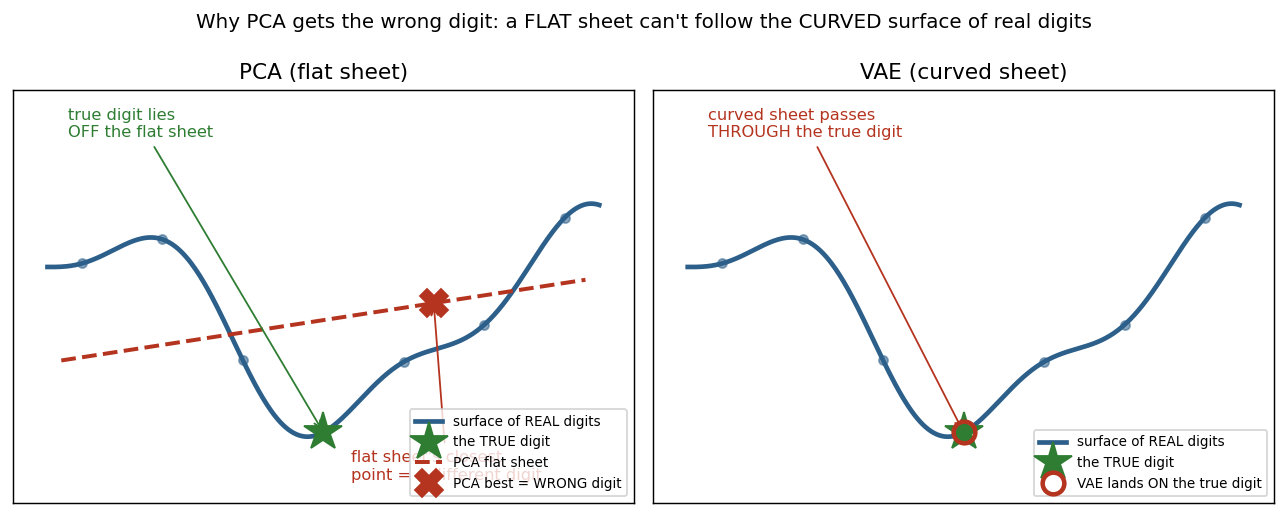
\includegraphics[width=0.98\textwidth]{fig_flat_vs_curved.png}
\caption{The flat-vs-curved problem (and why the VAE in Lesson 21 fixes it).
The blue wavy line is the surface of real digits; the green star is the true
digit, which sits \emph{on} it. \textbf{Left (PCA):} the red dashed line is
PCA's flat approximation; the true digit lies off it, and the flat sheet's
best available point (red X) is a \emph{different} digit. \textbf{Right (VAE):}
the curved sheet \emph{is} the digit surface, so it passes right through the
true digit.}
\end{figure}

\paragraph{Reason 2: many valleys (``multimodality'').} Recall (Lesson 5) that
several different digits can each explain the readings reasonably well. In our
``landscape'' picture (Lesson 12), that means the landscape has \emph{many
separate valleys} --- one near a plausible ``2,'' another near a plausible
``9,'' and so on --- all of them fairly low. Our downhill-walking search rolls
into whichever valley it happens to start nearest, and stops. It has no way to
know a better valley exists on the far side of a hill.

\begin{figure}[h]\centering
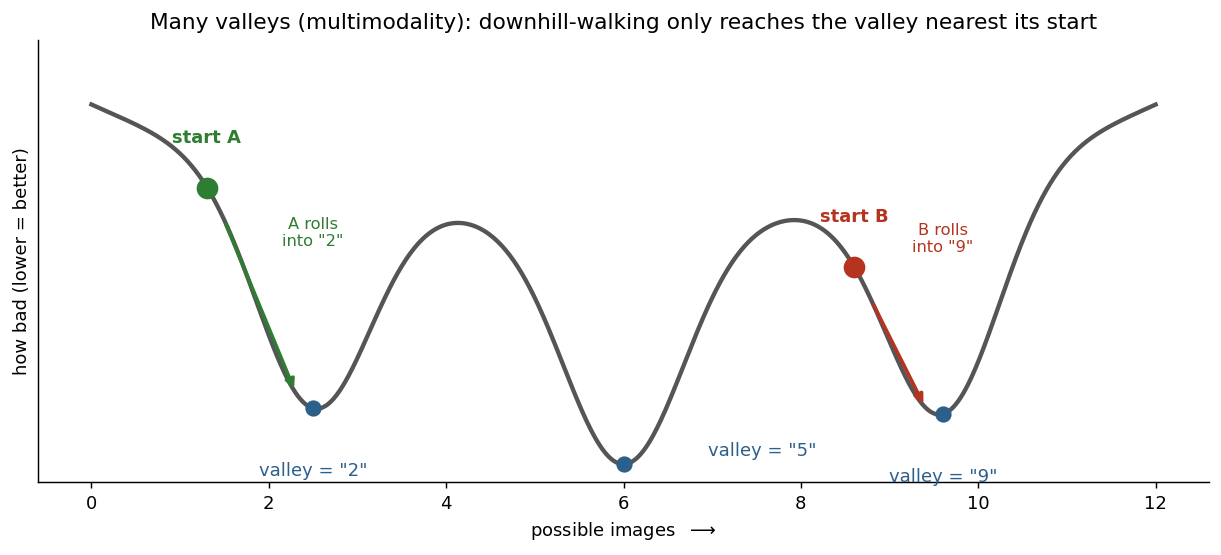
\includegraphics[width=0.95\textwidth]{fig_valleys.png}
\caption{The villain, drawn out. The curve is ``how bad each possible image
is'' (lower = better). It has several low valleys --- one near a plausible
``2,'' one near ``5,'' one near ``9'' --- because several digits roughly fit the
readings. A downhill-walking search rolls into whichever valley it starts
nearest (green vs.\ red) and stops there. It cannot tell that a different,
equally-good valley exists elsewhere.}
\label{fig:valleys}
\end{figure}

We proved this directly: when we \emph{started} the search at a ``2'' it
returned a ``2''; started at a ``5'' it returned a ``5''; started from a blank
average it drifted to a ``9.'' The data could not override the starting point
(see Figure~\ref{fig:initdigit}, which is the real-data version of the cartoon
in Figure~\ref{fig:valleys}). This ``many valleys, you only find the nearest''
phenomenon is called \textbf{multimodality}, and it is the central villain of
the whole project.

\begin{figure}[h]\centering
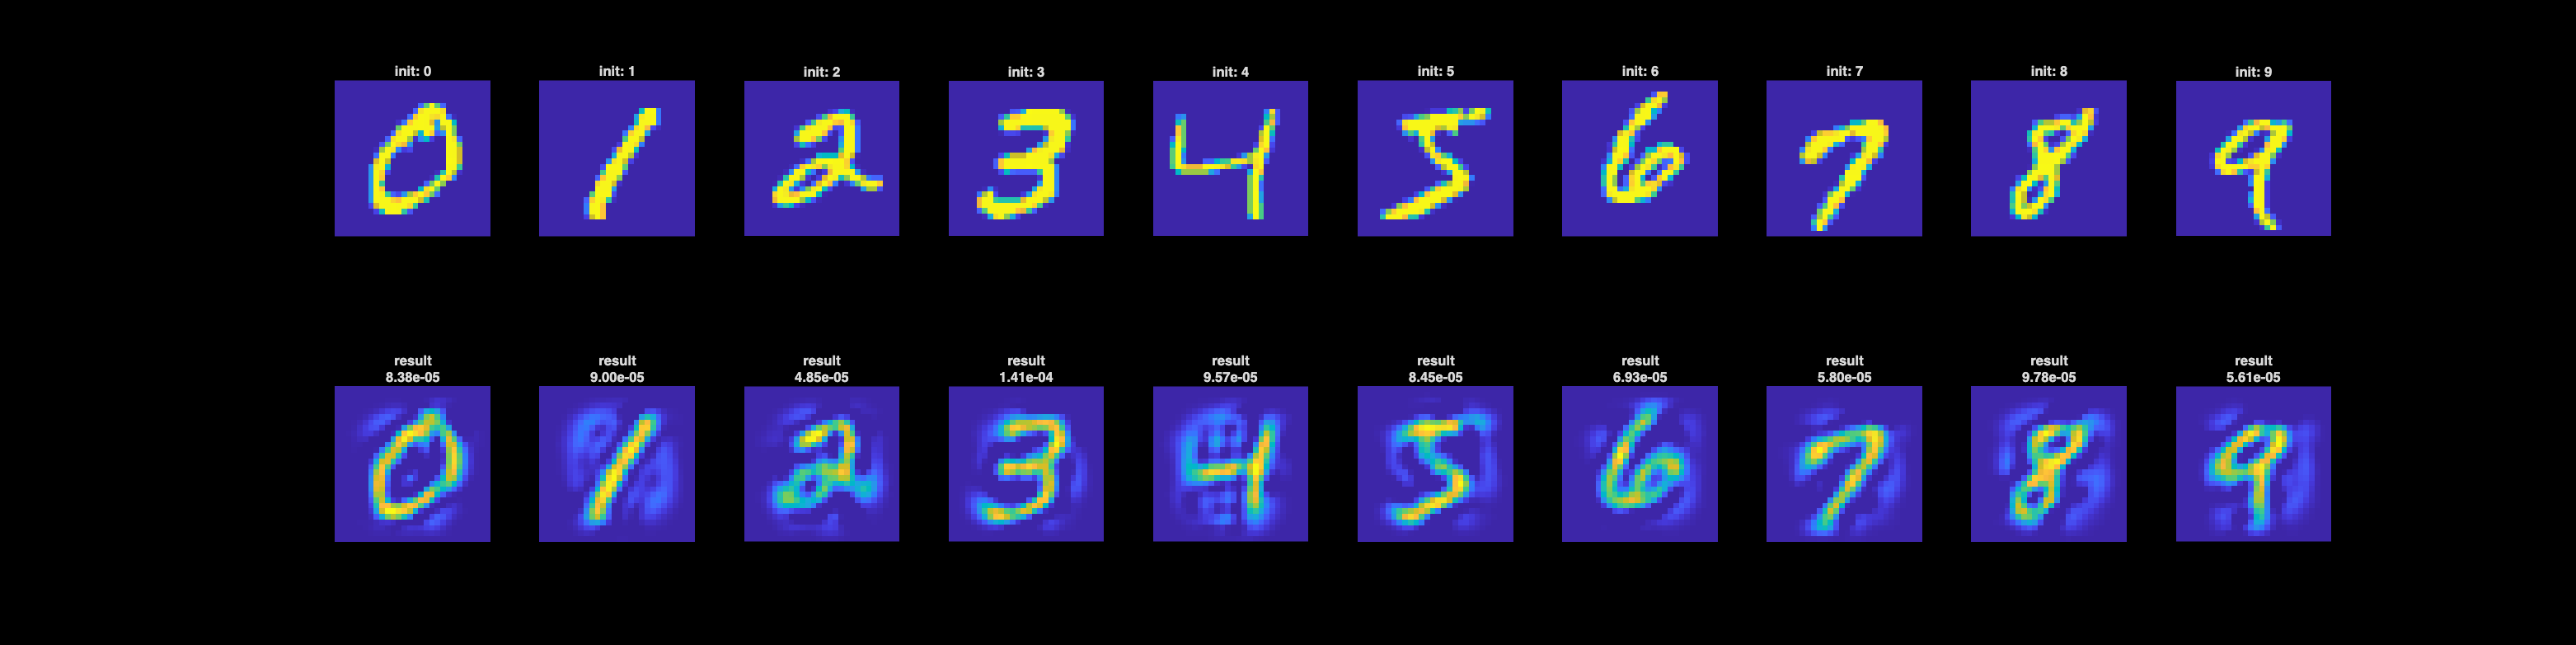
\includegraphics[width=0.95\textwidth]{diagnostic_initdigit.png}
\caption{Proof of ``many valleys.'' Top row: the digit we started the search
from. Bottom row: what it converged to. Each answer just resembles its own
starting point. The readings alone do not determine the digit; the starting
guess does.}
\label{fig:initdigit}
\end{figure}

\begin{key}
\textbf{Multimodality} = the landscape has many low valleys (many digits
roughly fit), and downhill-walking only finds the valley nearest where it
started. This is why a smarter \emph{prior} alone is not enough --- we also
need a smarter \emph{search} that does not get stuck in the wrong valley.
Hold this thought; it is the reason the winning method works.
\end{key}

\section{Lesson 21: The VAE --- a \emph{curved} sheet of digits}

PCA's weakness was that its sheet is flat. What if the ``building-block''
machine could bend, following the curved surface of real digits? That is what
a \textbf{VAE} (Variational Autoencoder) gives us. This is the piece that was
written incomprehensibly before, so we go slowly and define every word.

\paragraph{First: what is a neural network?} A neural network is just a
flexible \emph{function} --- a machine that takes some numbers in and gives some
numbers out --- built by stacking very simple steps. Each step does two things:
(1) \emph{mix} the incoming numbers (multiply them by weights and add them up
--- like PCA's ``mix the building blocks''), and (2) \emph{bend} the result
with a simple nonlinear squashing operation (for example, ``if a number is
negative, set it to zero''). Mixing alone can only ever make flat sheets;
adding the ``bend'' step at each layer is what lets the overall function curve.
Stack a few mix-then-bend steps and you get a function that can follow
complicated curved shapes.

\analogy{Mixing = stretching and rotating a sheet of dough (still flat).
Bending = folding the dough. Do ``stretch, fold, stretch, fold'' a few times
and you can shape the dough into almost anything. A neural network is
``mix, bend, mix, bend.''}

\paragraph{What is a ``latent code''?} We said any digit can be pinned down by
a short list of numbers (like PCA's 50 mixing amounts). For the VAE we call
that short list the \textbf{latent code}, written $z$. Think of $z$ as the
``coordinates'' of a digit on the curved surface of all digits.

\analogy{Every place on Earth's (curved) surface can be named by just two
numbers --- latitude and longitude --- even though Earth sits in 3D space.
Those two numbers are like the latent code: a short list of coordinates that
locates you on a curved surface.}

\paragraph{What is the ``decoder''?} The \textbf{decoder} is the part of the
VAE that takes a latent code $z$ (the coordinates) and produces the actual
$784$-pixel image (the point on the surface). Coordinates in, picture out.

\analogy{Type GPS coordinates into a map and it shows you the actual place.
The decoder is that map: latent code in, the digit it names comes out.}

\paragraph{How we trained it.} We showed the VAE all 60{,}000 MNIST digits and
let it learn a decoder such that (a) every real digit has some short latent
code that decodes back to it, and (b) decoding \emph{any} reasonable short
code produces a realistic-looking digit. After training we kept only the
decoder: our ``curved building-block machine.'' (We sanity-checked it by
decoding random codes --- out came clean digits, see
Figure~\ref{fig:vaesamples}.)

\begin{figure}[h]\centering
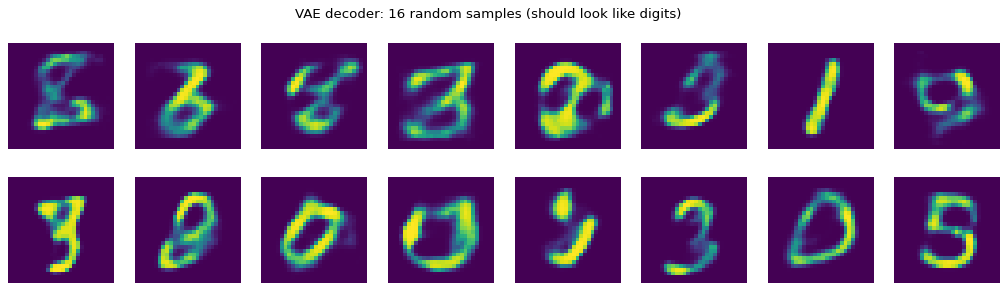
\includegraphics[width=0.9\textwidth]{vae_samples_preview.png}
\caption{Sanity check: feeding random latent codes into the trained decoder
produces realistic digits. This confirms the decoder really did learn the
``curved surface of digits.''}
\label{fig:vaesamples}
\end{figure}

\paragraph{How we used it to solve the inverse problem.} Same plan as PCA, but
with the curved machine. We search over the short latent code $z$, and for any
$z$ we (1) decode it into an image, (2) run the simulator $F$ to predict its
readings, (3) compare to the measured readings, and (4) nudge $z$ to make the
match better. ``Nudge $z$ in the downhill direction'' just requires passing
our usual downhill signal $J^\top r$ \emph{backward} through the decoder's
mix-and-bend steps to learn how each coordinate of $z$ should change. Passing
a downhill signal backward through a neural network's steps is a standard
procedure called \textbf{backpropagation} --- it is literally just the calculus
chain rule applied step by step, working from the output back to the input.

\analogy{Backpropagation is like tracing a problem back up an assembly line.
The final product is flawed (readings do not match). You walk backward
station by station asking ``how should the work at \emph{this} station change
to fix the final product?'' until you reach the very first station --- the
latent code. Then you adjust there.}

\textbf{What happened.} The VAE got the digit \emph{right} --- it recovered the
correct identity, the first method to do so --- because its curved surface
contains \emph{only} real digits and \emph{can} actually represent the true
one. It came out a little blurry only because our VAE was small and quick to
train. The crucial lesson, though, is not about blur. It is the comparison in
the next lesson.

\section{Lesson 22: The paradox --- the best ``score'' was the wrong answer}

Line up the three serious methods:

\begin{center}
\begin{tabular}{lcc}
\toprule
Method & data-match error (lower looks ``better'') & correct digit? \\
\midrule
TV (best generic) & $3.4\times10^{-4}$ & no (blob) \\
PCA (flat sheet) & $\mathbf{2.6\times10^{-5}}$ (the lowest!) & \textbf{no} (wrong digit) \\
VAE (curved sheet) & $6.1\times10^{-5}$ (higher) & \textbf{yes} (right digit) \\
\bottomrule
\end{tabular}
\end{center}

Stare at this. PCA had the \emph{lowest} error but gave the \emph{wrong}
digit. The VAE had a \emph{higher} error but gave the \emph{right} digit
(Figure~\ref{fig:two}). So ``lower error'' did \emph{not} mean ``better
answer.'' How can that be?

Because the problem is ill-posed (Part II), once you are matching the readings
about as well as the noise allows, squeezing the error even lower no longer
makes the picture more correct --- it just means you are bending the image to
chase meaningless measurement noise. A loose prior (PCA's flat sheet) is happy
to contort itself into a wrong digit if that shaves off a little error. A
tighter, more honest prior (the VAE's digit-only surface) refuses to do that,
so it keeps a slightly higher error but stays a real, correct digit.

\begin{key}
\textbf{The deepest lesson of the project:} for an ill-posed problem,
\emph{data-match error is not a measure of how correct your picture is}. Below
the noise level, lower error can actually mean a \emph{worse} picture. What
really matters is the \emph{quality of your prior}. This is exactly why the
winning method focuses everything on having the strongest possible prior.
\end{key}

\begin{figure}[h]\centering
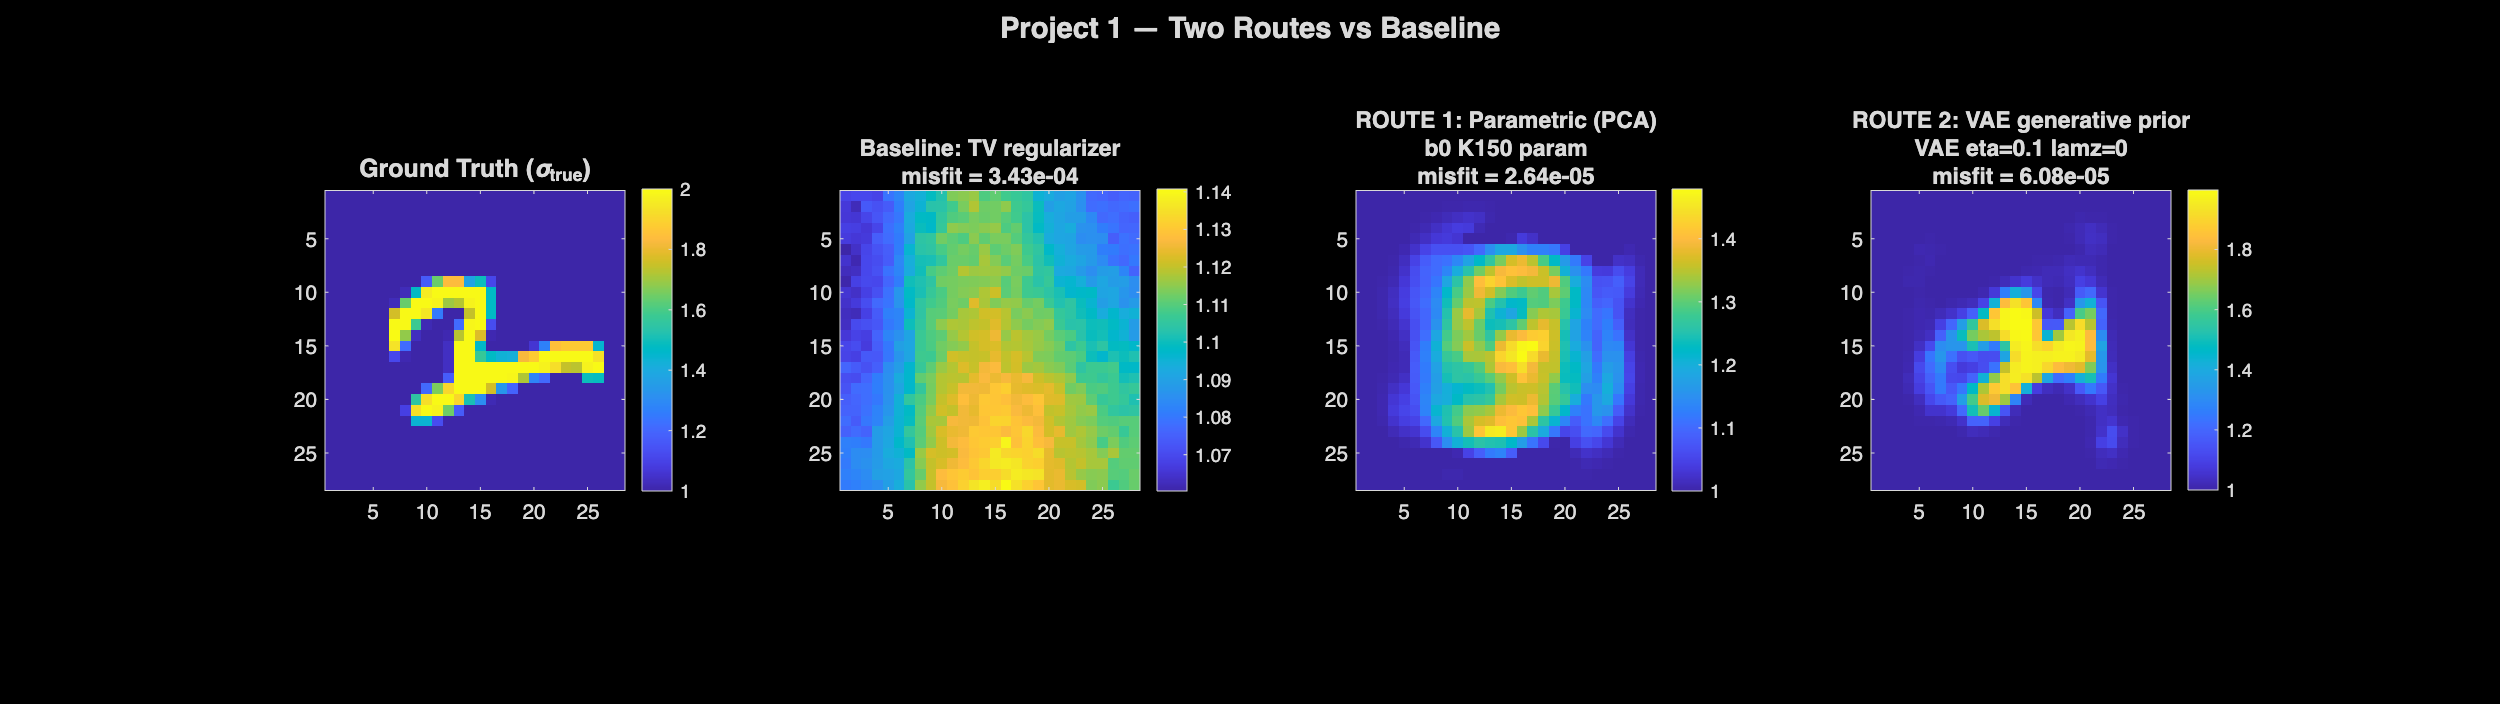
\includegraphics[width=0.95\textwidth]{two_route_comparison.png}
\caption{Left to right: the true digit; TV (blurry blob); PCA (lowest error
but the \emph{wrong} digit); VAE (higher error but the \emph{correct} digit).
Lower error did not mean a better answer.}
\label{fig:two}
\end{figure}

\begin{intuition}
\textbf{Explain it to a friend in 60 seconds (Part V).} ``We tried priors from
dumb to smart. `Keep it small/smooth/sparse' just gives blobs --- they don't
know what a digit is. So we learned a prior from the 60{,}000 real digits.
A \emph{flat} learned prior (PCA) gave a crisp but \emph{wrong} digit, because a
flat sheet can't follow the curved surface of real digits, and because
downhill-walking gets stuck in the nearest of many valleys. A \emph{curved}
learned prior (a small neural net, the VAE) got the digit \emph{right}. Big
lesson: the method with the lowest error gave the wrong answer --- so error
isn't the goal; \emph{the quality of the prior is.}''
\end{intuition}

%==============================================================
\part*{Part VI --- The method that actually worked}
\addcontentsline{toc}{section}{Part VI --- The method that actually worked}
%==============================================================

Everything so far has been building to this. We now have two lessons in hand:
(1) use the strongest possible prior (Lesson 22), and (2) avoid getting stuck
in the wrong valley (Lesson 20). The winning method does both, and it is
beautifully simple.

\section{Lesson 23: The strongest prior --- ``it is literally one of these 60{,}000''}

Re-read the project statement: the hidden image is ``very similar to one of
the MNIST samples.'' We had been treating this softly (``looks digit-ish,''
``lives on the digit surface''). The \emph{strongest} honest reading is much
sharper:

\begin{center}
\emph{The answer is essentially one of the 60{,}000 actual MNIST images we
already have.}
\end{center}

This is the most powerful prior possible: instead of allowing any digit-like
image, it allows only the 60{,}000 specific real images we hold in our hand.
There is no static-junk to worry about, no flat-vs-curved-sheet issue --- the
candidate answers are 60{,}000 genuine, clean digits.

\section{Lesson 24: Template matching --- just try all 60{,}000}

If the answer is one of 60{,}000 known images, the strategy writes itself:
\begin{quote}
For each of the 60{,}000 images, run the forward simulator $F$ to predict
\emph{what readings that image would produce}, and compare those predicted
readings to the readings we actually measured. Whichever image's predicted
readings match best \emph{is the answer.}
\end{quote}
We call each candidate image a \emph{template}, and the procedure
\textbf{template matching}. Concretely, for template number $i$ we compute its
data-match error $\tfrac12\norm{F(\text{template}_i)-y_{\text{obs}}}^2$, and we
keep the template with the smallest error.

\begin{figure}[h]\centering
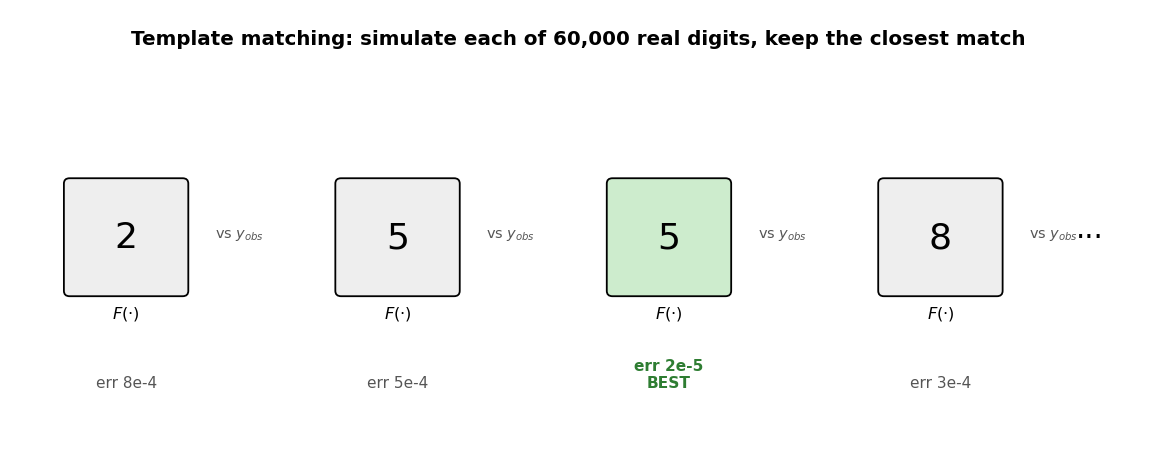
\includegraphics[width=0.95\textwidth]{fig_template_match.png}
\caption{Template matching. Take each real MNIST digit, run the simulator $F$
to predict the readings it would produce, and compare to the measured readings
$y_{\text{obs}}$. Keep the one whose predicted readings are closest (smallest
error). Because we check \emph{every} candidate, there is no ``nearest valley''
to get stuck in.}
\end{figure}

\paragraph{This is not a hack --- it is the mathematically optimal answer.}
Here is the satisfying part. Plug the prior ``the answer is one of these
60{,}000'' into the combine-data-and-prior recipe from Lesson 11. Because the
prior allows \emph{only} those 60{,}000 images, the recipe reduces to: among
those 60{,}000, pick the one with the smallest data-match error. That is
\emph{exactly} template matching. In other words, template matching is the
provably best possible estimate under this prior --- not a shortcut, but the
right answer.

\begin{intuition}
Another way to see it: each template has a ``measurement fingerprint'' (the
readings it would produce). Template matching just finds the template whose
fingerprint is closest to the fingerprint we actually measured. It is
``find the nearest match'' --- the same idea as recognizing a song from a short
clip by comparing fingerprints.
\end{intuition}

\paragraph{Why this dodges the wrong-valley trap.} The downhill-walking
methods (PCA, VAE) only ever explore \emph{one valley} --- the one near their
start --- so they can be fooled into the wrong digit. Template matching
\emph{checks all 60{,}000 candidates}. It looks in every valley at once. There
is no ``nearest valley'' to get stuck in, because we simply try everything.
This is precisely the fix for the multimodality villain of Lesson 20.

\paragraph{What we found.} The eight best-matching templates were almost all
the \emph{same digit and shape} (see Figure~\ref{fig:top8}) --- a strong
agreement that tells us the digit identity with high confidence. The single
best template matched the readings about 30 times better than the best PCA/VAE
attempts.

\begin{figure}[h]\centering
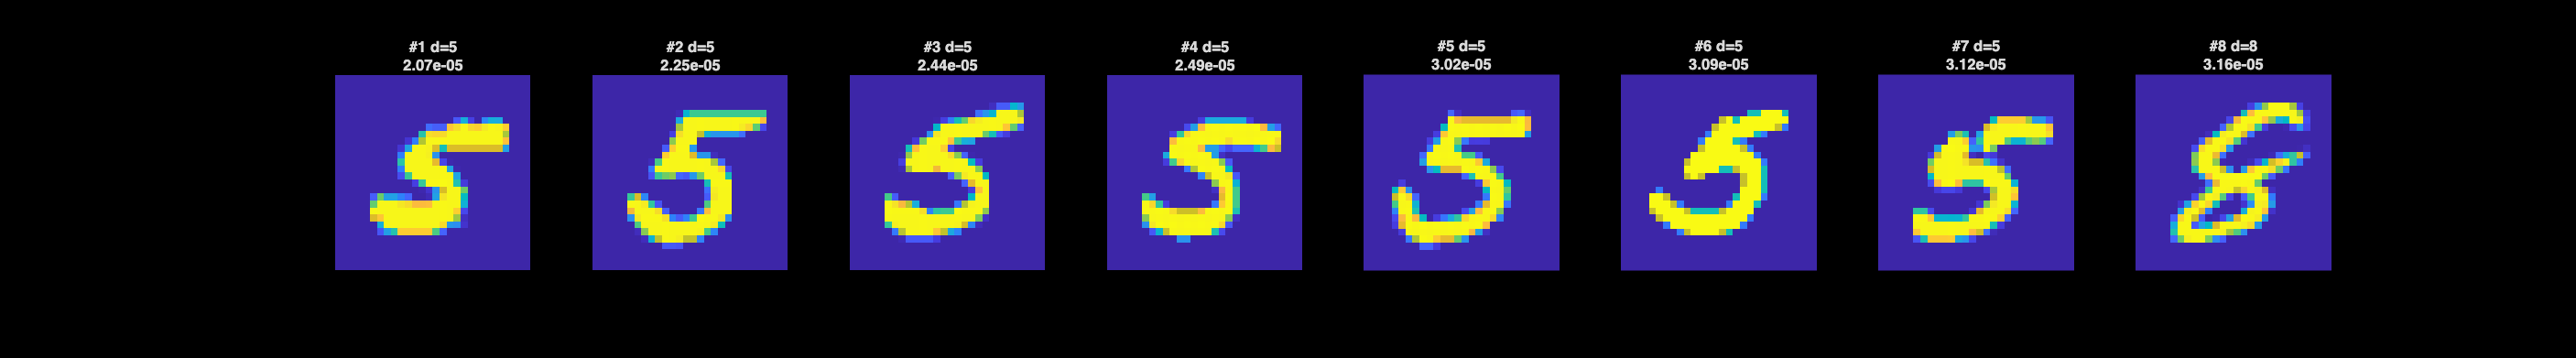
\includegraphics[width=0.95\textwidth]{exact_template_top8.png}
\caption{The eight templates whose simulated readings best match the data.
Seven of eight are the same digit in nearly the same pose --- strong agreement,
high confidence in the identification.}
\label{fig:top8}
\end{figure}

\section{Lesson 25: Why we simulate each template exactly (instead of approximating)}

A tempting shortcut: simulating $F$ for all 60{,}000 templates sounds like a
lot, so why not \emph{approximate} each template's readings with a quick
formula instead of a full simulation? We tried it. It failed --- it even
picked the wrong digit --- because the approximation is only accurate when the
hidden feature is faint, and our digits are \emph{strong} (high contrast). For
strong features the quick formula is too far off to trust.

The good news: a single exact simulation is cheap (it is one solve of a sparse
system), so simulating all 60{,}000 takes only about 15 minutes, and it is
embarrassingly easy to split across processors. We happily paid that price for
accuracy. \emph{Lesson: when in doubt, simulate exactly --- approximations can
quietly give you the wrong answer.}

\section{Lesson 26: Refinement --- polishing the winner}

Template matching hands us the best of the 60{,}000 real digits. But the true
hidden digit might differ \emph{slightly} from every single training image
(maybe a stroke is a touch thicker). So we add a quick polishing step.

Starting \emph{from} the winning template, we run our ordinary downhill search
(Lesson 14) on the data term. Here is why this is now safe, whereas before it
got stuck: template matching has already placed us \emph{in the correct
valley} (the right digit). Within that one valley there is just a single
bottom to roll down to --- no other digits to be lured toward --- so plain
downhill walking simply sharpens the details. It is no longer fighting
multimodality; that battle was already won in Lesson 24.

This polishing drove the data-match error down by more than tenfold (from
about $2\times10^{-5}$ to about $2\times10^{-6}$) while keeping a clean,
correct digit (Figure~\ref{fig:answer}).

\begin{intuition}
\textbf{The two stages, together.} Stage 1 (template matching) solves the
\emph{hard} part --- which digit? --- by a global search that cannot get stuck.
Stage 2 (refinement) solves the \emph{easy} part --- the exact shape --- by
local polishing in the now-correct valley. Splitting the job this way is the
whole trick. The methods that failed tried to do both at once with a single
downhill walk, and got trapped.
\end{intuition}

\begin{figure}[h]\centering
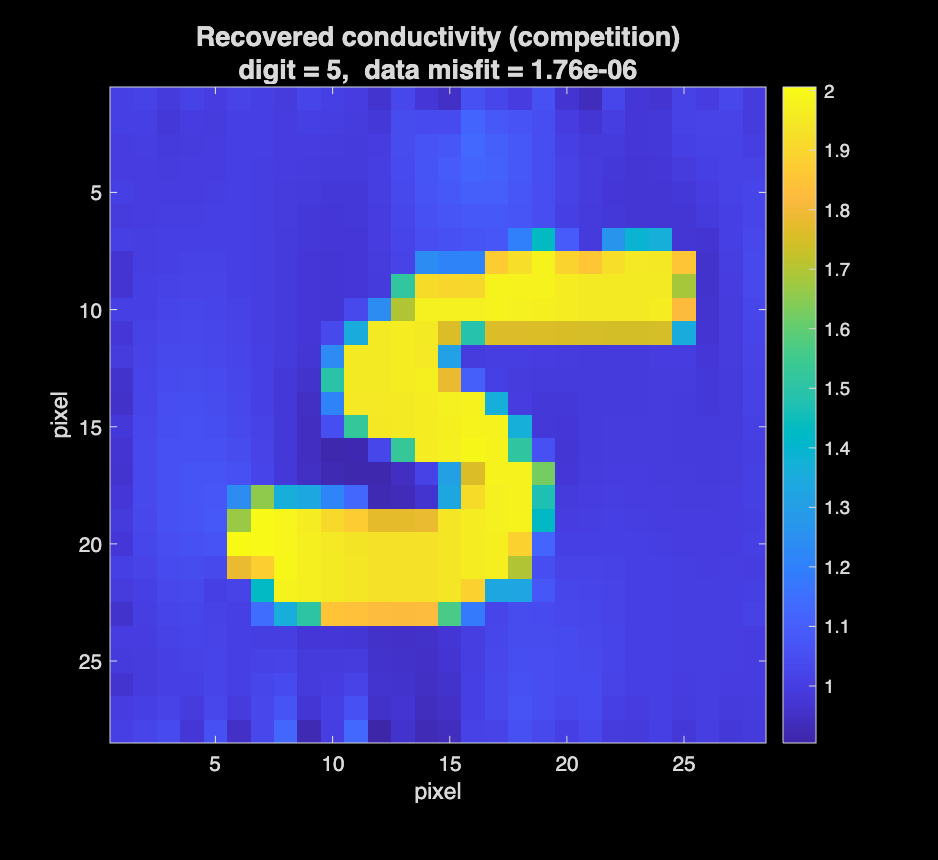
\includegraphics[width=0.72\textwidth]{competition_answer.png}
\caption{Left: the best template from Stage 1 (a clean, real MNIST digit).
Right: the Stage-2 refined result --- a clean, correct digit matching the
readings about 200 times better than the original TV baseline.}
\label{fig:answer}
\end{figure}

\section{Lesson 27: The whole method on one page}

\begin{mdframed}
\textbf{Goal.} From the measured readings $y_{\text{obs}}$, recover the hidden
digit.

\smallskip
\textbf{Stage 1 --- identify the digit (global search).}
For each of the 60{,}000 MNIST templates: run the simulator $F$ to predict its
readings, and measure how far those are from $y_{\text{obs}}$. Keep the
template with the smallest gap. \emph{(This is the mathematically optimal
choice under the prior ``the answer is one of these images,'' and because it
checks all candidates it cannot get stuck on the wrong digit.)}

\smallskip
\textbf{Stage 2 --- polish (local search).}
Starting from that winning template, take small downhill steps (with momentum)
to reduce the data-match error further, keeping conductivity non-negative.
\emph{(Safe now, because Stage 1 put us in the correct valley.)}

\smallskip
\textbf{Output.} A clean, correct reconstruction of the hidden digit.
\end{mdframed}

\textbf{Why it beats everything else, in one sentence:} it uses the strongest
possible prior (the real images themselves) \emph{and} searches globally so it
never gets trapped in the wrong digit --- the two things every other method
lacked.

\begin{intuition}
\textbf{Explain it to a friend in 60 seconds (Part VI).} ``The project says the
answer is basically one of 60{,}000 known digit pictures. So instead of
blindly searching, we just \emph{try all 60{,}000}: simulate the readings each
one would produce, and keep the closest match. That's actually the
mathematically optimal answer under that assumption, and because we check
everything we can't get stuck on the wrong digit. Then we polish the winner
with a little downhill tuning. Clean, correct digit --- done.''
\end{intuition}

\section{Lesson 28: Does it actually work? A 10-digit stress test}

It is fair to ask whether we simply got lucky on one digit. To check, we ran the
\emph{exact same method} on ten brand-new digits and watched whether it recovered
each one.

\paragraph{The honest setup.} MNIST ships as two separate piles: 60{,}000
\emph{training} images and 10{,}000 \emph{test} images the method never sees.
We used the training pile as the dictionary (the prior), then took one
\emph{test} digit of each kind, 0 through 9, simulated its readings with $F$, and
asked the method to recover it. Because the test digits are not in the
dictionary, the method cannot cheat by matching a digit to a copy of itself; it
must identify the \emph{kind} of digit from the readings alone.

\begin{figure}[h]\centering

\includegraphics[width=0.98\textwidth]{validation_0to9.png}
\caption{Ten unseen digits put through the method. \textbf{Top:} the true
(unseen) digit. \textbf{Middle:} the dictionary template Stage 1 picked --- the
number above each is the digit it identified, green when correct, red when wrong.
\textbf{Bottom:} the refined reconstruction. Nine of ten are correct.}
\end{figure}

\paragraph{The result: 9 out of 10.} Every digit came back correct except one,
where an unseen 5 was mistaken for a 6. That single miss is worth understanding,
because it \emph{confirms} the lessons rather than undermining them:

\begin{itemize}[leftmargin=2em]
\item \textbf{It was the least-confident case.} Recall from Lesson 8 that the
data-match error is really a confidence score. The mistaken 5 had the
\emph{worst} Stage-1 error of all ten (about $6\times10^{-5}$, versus roughly
$1$--$3\times10^{-5}$ for the rest). The method was already ``unsure'' there,
exactly as the theory predicts.
\item \textbf{That handwritten 5 genuinely resembles a 6.} Its lower half curls
into a near-closed loop. With only part of the training set in play, the closest
\emph{reading} happened to come from a 6. This is the shadow problem of Lesson 5
made concrete: two different shapes casting almost the same shadow.
\item \textbf{The competition 5 is pinned down, not a coin-flip.} On the real
data the \emph{top eight} matches were seven 5's and a single 8 --- the leading
candidates overwhelmingly agree, which is the signal that the digit is truly
identified. The unseen-5 miss was the opposite: a near-tie a 6 won by a hair.
Agreement among the top matches is what tells us the competition answer is solid.
\end{itemize}

\begin{intuition}
\textbf{Why this matters for the talk.} If someone asks ``how do you know your 5
is right and not a fluke?'', this is the answer: the same method recovers 9 of 10
\emph{unseen} digits, and on the competition data the top matches nearly all
agree on 5. The lone miss is the method honestly flagging its own uncertainty
--- which is exactly what a trustworthy method should do.
\end{intuition}

%==============================================================
\part*{Part VII --- Wrap-up}
\addcontentsline{toc}{section}{Part VII --- Wrap-up}
%==============================================================

\section{Lesson 29: The whole story, start to finish}

\begin{enumerate}[leftmargin=2em]
\item We want the hidden conductivity image from edge voltage readings
(Lessons 1--4).
\item It is \emph{ill-posed}: many images fit, and noise blows up --- so
matching the readings is not enough (Lessons 5--6).
\item We turn ``recover the image'' into ``minimize (data mismatch) $+$
(prior penalty),'' where the data part comes from bell-curve noise and the
prior part encodes what an answer should look like; a regularizer \emph{is} a
prior (Lessons 7--11).
\item A computer minimizes this by walking downhill, using the gradient
$J^\top r$ with momentum (Lessons 12--14).
\item Generic priors (small / sparse / few-edges) give blobs; a learned
\emph{flat} prior (PCA) gives a clean but \emph{wrong} digit; a learned
\emph{curved} prior (VAE) gives the \emph{right} digit --- teaching us that
prior quality, not data-match error, is what matters
(Lessons 15--22).
\item The strongest prior is ``the answer is one of the 60{,}000 real
images.'' Under it, the optimal method is to \emph{try them all} (template
matching) --- a global search that nails the digit without getting trapped ---
and then \emph{polish} the winner. That cleanly recovers the digit
(Lessons 23--27).
\end{enumerate}

\section{Lesson 30: How this connects to Project 2 (diffusion)}

Our winning prior is powerful but rigid: it can only return one of the
60{,}000 images (plus a little polish). It also returns a \emph{single} answer,
even though we saw the data can genuinely be consistent with more than one
digit.

Project 2 upgrades the prior with a \textbf{diffusion model} --- think of it as
a vastly more capable version of the VAE's ``curved surface of digits,'' able
to generate brand-new realistic digits, not just reproduce stored ones. Better
still, it can produce \emph{several} different plausible answers (sampling the
``many valleys'' honestly, instead of forcing one). And the way it folds in the
measurements is by using our exact same downhill signal $J^\top r$ at each
step. So Project 2 is the natural sequel: same forward simulator, same
data-match gradient, but a smarter, generative prior and a fairer way to
handle multiple possible answers.

\section{Lesson 31: A suggested way to present this}

A clean 10--12 minute talk:
\begin{enumerate}[leftmargin=2em]
\item \textbf{Hook:} ``We recovered a handwritten digit from 1900 voltage
readings around the edge of a box.'' Show the final digit.
\item \textbf{Setup:} forward (easy) vs.\ inverse (hard); one image
$\leftrightarrow$ 1900 readings.
\item \textbf{Why hard:} ill-posed --- many images fit, noise blows up (the
shadow analogy lands well).
\item \textbf{The framework:} minimize (data match) $+$ (prior); and the punch
line that \emph{a regularizer is just a prior}.
\item \textbf{What we tried:} generic $\to$ blob; PCA $\to$ clean but wrong
digit; VAE $\to$ right digit. Deliver the paradox: \emph{lowest error was the
wrong answer} (Figure~\ref{fig:two}).
\item \textbf{The villain:} multimodality --- many valleys, downhill gets
stuck (Figure~\ref{fig:initdigit}).
\item \textbf{The fix:} strongest prior + global search = template matching
(show the top-8 agreement, Figure~\ref{fig:top8}); then polish
(Figure~\ref{fig:answer}).
\item \textbf{Takeaway:} prior quality beats error-chasing; and a one-line
tease of Project 2.
\end{enumerate}

\paragraph{Five questions you will probably get --- and short answers.}
\begin{itemize}[leftmargin=2em]
\item \emph{Isn't ``try all 60k'' just cheating/lookup?} No --- it is the
provably optimal estimate under the stated prior, and Stage 2 refines beyond
any stored image. The ``lookup'' is a principled \emph{global} search that the
downhill methods cannot do.
\item \emph{Why not approximate each template to go faster?} The digits are
high-contrast, so the fast approximation is inaccurate and even picked the
wrong digit. Exact simulation is cheap enough.
\item \emph{What if the true digit isn't in the 60k?} Stage 1 still finds the
closest real digit (identity confirmed by the top-8 agreement), and Stage 2
moves off the template to fit the exact shape.
\item \emph{Why did the lowest-error (PCA) result look wrong?} Below the noise
level, lower error just means chasing noise; a loose prior exploits that with
a wrong image. Error is not correctness.
\item \emph{Where does $J^\top r$ come from?} It is the downhill direction of
the data term --- a vote where each reading pushes on the pixels it affects,
weighted by how wrong that reading currently is. It is computed efficiently by
the adjoint trick, already inside the simulator.
\end{itemize}

\end{document}
